\documentclass[a4paper, 10pt, superscriptaddress, nofootinbib, showkeys, notitlepage]{revtex4-1}
%!TEX encoding = UTF-8 Unicode
%%%%%%%%%%%%%%%%%%%%
\usepackage[english]{babel}
\usepackage{amsmath, amssymb, amsfonts, amscd, amsthm}
\usepackage[a4paper,top=3.5cm,bottom=3cm,left=2.5cm,right=2.5cm,bindingoffset=5mm]{geometry}
\usepackage{dsfont}
\usepackage{mathrsfs}
\usepackage{stmaryrd}
\usepackage[utf8x]{inputenc}
\usepackage{indentfirst}
\usepackage{microtype}
\usepackage{graphicx}%insert figures
\usepackage{float}
\usepackage[margin=2cm, labelfont=it, justification=justified]{caption}
\usepackage{textcomp}
\usepackage{array, booktabs}
\usepackage[colorlinks=true, linkcolor = blue, citecolor= red, urlcolor= red]{hyperref}
\usepackage{tikz, tikz-cd}
\usetikzlibrary{arrows, calc, shapes, fit, matrix, decorations.pathreplacing, decorations.markings, decorations.pathmorphing, positioning, fadings, patterns, chains}
\usepackage[all]{xy}
\usepackage{stackengine,scalerel}
\usepackage{mathtools}
\usepackage{numprint}
\npthousandsep{\,}
\usepackage{cleveref}


\tikzstyle{vecArrow} = [thick, decoration={markings,mark=at position
   1 with {\arrow[semithick]{open triangle 60}}},
   double distance=1.4pt, shorten >= 5.5pt,
   preaction = {decorate},
   postaction = {draw,line width=1.4pt, white,shorten >= 4.5pt}]
\tikzstyle{innerWhite} = [semithick, white,line width=1.4pt, shorten >= 4.5pt]

%%%%%%%%%%%%%%%%%%%%%%%%%%%%%%%%%

%%%%%%Command redefinitions%%%%%%%

%%%%%%%%%%%%%%%%%%%%%%%%%%%%%%%%%

%%%%%%%%%%%%%%%%%%%%%Abstract environment definition%%%%%%%%%%%%%%%%
%\renewenvironment{abstract}{\begin{center}\begin{minipage}{0.77\textwidth}\rule{\textwidth}{0.04em}\\[0.4em]\small\textbf{\abstractname~|}}{\par\rule{\textwidth}{0.04em}\end{minipage}\end{center}}
%%%%%%%%%%%%%%%%%%%%%%%%%%%%%%%%%%%%%%%%%%%%%%%%%%%%

%
%%
%%%
%%%%%%
%%%%%%%%%
%%%%%%%%%%%%
%%%%%%%%%
%%%%%%
%%%
%%
%
\begin{document}

%%%%%%Authors details%%%%%%

\author{Oscar de Felice}
%%
	\affiliation{via dei Genovesi 92, 09124 Cagliari, Italy}
%%
	{\let\thefootnote\relax\footnote{\hspace{-4ex}\textsuperscript{1}\emph{e-mail}: \href{mailto:oscar.defelice@gmail.com}{oscar.defelice@gmail.com}}}
%%%
\author{Gustavo de Felice}
%%
	\affiliation{via Silvio Pellico 12, 84073 Sapri, Italy}
%%
	{\let\thefootnote\relax\footnote{\hspace{-4ex}\textsuperscript{2}\emph{e-mail}: \href{mailto:gustavo@dottordefelice.it}{gustavo@dottordefelice.it}}}
%%%


%%%%
%%%%%%%%%%%%%%%%%%%%

\date{\today}
%
%%
%%%
%%
%
%
%%%%%%Title%%%%%%%%%%%%
\title{A supervised image recognition approach to diagnose dental diseases}
%%%%%%%%%%%%%%%%%%%%
%
%%%%%%%%%%%%
\begin{abstract}
%
	The main goal of this document is to describe the idea of image recognition to determine whether a patient may have some odontoiatric disease.
	This falls in the framework of the so-called computer aided diagnosis (\textsc{CAD}).
	Briefly, we aim to use a machine learning approach, training an image recognition algorithm over an image database, labelled with the diseases and use the fitted model to predict whether a new image has the features characterising a specific illness. The idea is to give suggestions to doctors alerting them when an image is found with a high probability of a disease.
	The approach is general, however, in this document we want to focus on the \emph{periodontal disease} or \emph{periodontitis} and analyse such cases.
%
\end{abstract}
%%%%%%%%%%%%%
%
\maketitle
%
%%

\section*{Introduction}
	%	
	An important issue to face since the birth of image recognition techniques is the detection and classification of objects in digital images. 
	Obviously, objects can be classified by several aspects, \emph{e.g.} colours, textures, shapes, position within images, etc.
	
	Recently, there have been several satisfying examples of the use of such approach~\cite{castanon2007, Arena2003}. 
	Even back to the early 2000's, one can find contributions to the applications image recognition to medical diagnostic systems~\cite{Comaniciu1999, Jain2000}.
	%
	%
	%%%%%
	%%%
	%%
	%
\section{A warm-up example: cats vs dogs recognition}
	%
	Just to illustrate the method, we want to describe a simple image recognition algorithm. 
	The basic idea is to detect whether in pictures there is a cat or a dog.
	This is a typical example of supervised online learning algorithm, easy to explain and rich enough to present several interesting features. 
	
	We are going to use of the notorious \href{https://www.kaggle.com/c/dogs-vs-cats}{Kaggle's cats vs dogs dataset}.
	This is made up by \numprint{25000} examples, evenly distributed, \emph{i.e.}
		%
		\begin{itemize}
			\item[] \numprint{12 500} images of cats;
			\item[] \numprint{12 500} images of dogs.
		\end{itemize}
		%
	Our goal is to describe the incremental learning procedure in this toy case, and then apply it to our medical case.
	%
	%
	%%%
	%%
	%
\subsection{Understanding how image recognition works}
	%
	Here, we give a brief description of the major points of an image recognition algorithm.
	Figure~\ref{fig:cat-vs-dog} illustrates the scheme.
		%
		\begin{figure}[h]
  			\includegraphics[width=.7\linewidth]{Images/cat-vs-dog.jpg}
 			\caption{Working scheme of the image recognition algorithm.}
 			\label{fig:cat-vs-dog}
		\end{figure}
		%
	We have a dataset made up of images, objects that can be thought as a matrix where each entry position corresponds to a pixel and each entry value to the colour of that pixel.
	
	The algorithm can be split into two phases:
		%
		\begin{enumerate}
			\item Feature extraction.
			\item Neural network training.
		\end{enumerate}
		%
	The output of the algorithm is a \emph{trained model} as one can see in figure~\ref{fig:scheme}.
	
	The trained model can be used to make predictions.
	Indeed, the trained model is nothing else than a law with optimised values of parameters, to get as close as possible to its experience, \emph{i.e.} what it learnt from the dataset.
		%
		\begin{figure}[h]
		\centering
			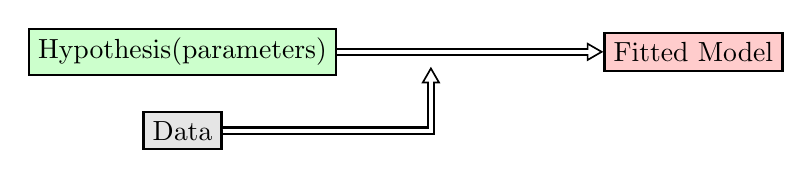
\begin{tikzpicture}[thick]
 				 \node[draw,rectangle, fill = green!20] (a) {Hypothesis(parameters)};
 				 \node[inner sep=0,minimum size=10,right= 1 cm of a] (k) {}; % invisible node
 				 \node[draw,rectangle,right= 2 cm of k, fill = red!20] (b) {Fitted Model};
 				 \node[draw,rectangle,below of=a, fill = gray!20] (c) {Data};

  				% 1st pass: draw arrows
  				\draw[vecArrow] (a) to (b);
  				\draw[vecArrow] (c) -| (k);

  				% 2nd pass: copy all from 1st pass, and replace vecArrow with innerWhite
  				\draw[innerWhite] (a) to (b);
  				\draw[innerWhite] (c) -| (k);

  				% Note: If you have no branches, the 2nd pass is not needed
			\end{tikzpicture}
			\caption{Working scheme of a machine learning algorithm. Data are used to fit parameters }
			\label{fig:scheme}
		\end{figure}
		%
	%
	%
	%%%%%
	%%%
	%%
	%
\section{Overview of diagnostic systems based on automatic image recognition}
	%
	In this section we review the general scheme of diagnostic systems based on a machine learning approach. 
	In particular, we are going to expose the working mechanism of image recognition algorithms applied to medical diagnosis.
	
	First, we access to database. 
	It is important fort the sake of precision the algorithm to have access to a large number of images.
	The training phase is the one where \emph{weights} of the neural network are tuned.
	We make use of a convolutional neural network (\textsc{cnn}) for features extraction and then for image recognition, as illustrated in figure~\ref{fig:cad-cnn}.
	
		%
		\begin{figure}[h]
  			\includegraphics[width=.7\linewidth]{Images/CNN.png}
 			\caption{Training of the convolutional neural network for computer aided diagnosis.}
 			\label{fig:cad-cnn}
		\end{figure}
		%
	We will be more precise about these technical details in a future version of this document.
	%
	%
	%%%
	%%
	%
%\subsection{Shape characterisation}
%	%
%	Mathematically, images can be thought as sets of connected points in a two-dimensional space $\mathcal{F}$, often (and also here) approximated in a discrete binary space.
%	People do not perform image classification directly on $\mathcal{F}$, since this task is computationally really expensive ($\sim \mathcal{O}(n^2)$), where each image is made up by $n$ pixels.
%	The representation of an image can be modified by an image transformation, by mapping the space $\mathcal{F}$ to a -- typically smaller -- feature space $\mathcal{F}'$.
%	
%	%
	%
	%%%%%
	%%%
	%%
	%
\section{The algorithm ingredients}
	%
	The aim of this section is to go in depth and describe how the algorithm works.
	However, here we want to give an introductory scheme, playing the role of a summary.
	The whole process can be split into the following steps
		%
		\begin{enumerate}
			\item Collecting images and labelling them to form the dataset.
			\item Train a neural network to tune the model parameters on the dataset images.
			\item Implement an online learning algorithm to update model parameters with new information coming with new images.
		\end{enumerate}
		%
	
	%
	%%%
	%%
	%
\subsection{Overview of a supervised learning algorithm to recognise diseases}
	%
	As in the case of face recognition we need a large corpus of images. 
	One can associate a label to each image indicating the diagnosis.
	For the moment being, to keep the system simple, we want just to add the ``yes/no'' label identifying the presence or absence of periodontitis.
	One can see figure~\ref{img:rxyes} for an illustration of such a flow.
	
		%
		\begin{figure}[h]
			\centering
			\begin{tikzpicture}
				\node[inner sep=0pt] (RX) at (0,0) {\includegraphics[width=.15\textwidth]{Images/Z14_000.png}};
				\node[inner sep=0pt] (RXlabeled) at (5,-6) {\includegraphics[width=.15\textwidth]{Images/Z14_000.png}};
				\node[inner sep=0pt] (label) at (3,-6) {\textcolor{red}{\textsc{Label \textbf{Y}}}};
				\draw[->,thick] (RX.south east) -- (RXlabeled.north west)
    					node[midway,fill=white] {Is the patient affected by periodontitis?};
				\draw[red,thick,dotted] ($(label.north west)+(-0.3,2.)$)  rectangle ($(RXlabeled.south east)+(0.3,-0.6)$);
			\end{tikzpicture}
			\caption{	Periodontitis image labelling.\\%
					Each image is decorated by a label indicating whether the periodontal disease is present or not.
					This will give the algorithm the information about how a radiography of a periodontitis patient should look like.}
			\label{img:rxyes}
		\end{figure}
		%
	%
	%
	%%%
	%%
	%
\subsection{The database}
	%
	Currently, we plan to use the provate database of radiograph images of \textsc{dr Gustavo de Felice}, acknowledging him for the courtesy.
	However, any contribution on this side is precious, so we plan to have access to further images to make the corpus big enough to guarantee good accuracy of the classification algorithm.
	
	Images are collected and labelled with the appropriate response, according to the periodontitis presence.
	We split them into training set and test set with a ratio $70/30$.
	Making use of the test set, we are able to calculate accuracy, recall and other classification metrics allowing us to evaluate how good the algorithm is performing.
	%
	%
	%%%
	%%
	%
\subsection{Training a neural network}
	%
	Once the labelling procedure is completed and the database completely set, one has to perform a model training over the whole dataset.
	This produces a fitted model, with some fixed values of parameters, allowing us to make predictions.
	At this stage, one can perform a metric measure, to give a score to the fitted model.
	%
	%
	%%%
	%%
	%
\subsection{Online learning}
	%
	Once the database is completely labelled and set, one can start evaluating new radiograph images.
	We are now in a new regime of machine learning, the so called \emph{online learning} or \emph{incremental learning}.
	This is a machine learning regime where a model learns one observation at a time.
	This is in contrast to batch learning we set before, in the initial stage where all the data is processed in one go. 
	Incremental learning is desirable when the data is too big to fit in memory, or simply when you want to streaming data.
	The last is our case, where we will have a stream of images coming each time a doctor takes a new radiography.
	
	Concretely, the model will evaluate one new image, giving an expected diagnosis. 
	The doctor will check whether the diagnosis is correct and giving an approval, to add the new image to the dataset.
	The model will update its parameters to take into account the new image.
	In this way the dataset will increase and accuracy will improve.
	%	
	%%%%%
	%%%
	%%
	%
%\section{Things to know}
%	%
%	
%	%
%	%%%
%	%%
%	%
%\subsection{Labelling the online dataset}
%	%
%	This is a responsibility of the doctor. When the algorithm will be up and running, the image will be evaluated, then a window will pop out on the screen suggesting the presence of the disease. 
%	The doctor will have a suggestion and he can accept or refuse the diagnosis. This will add the image to the database with a proper label according to the human answer.
%	
%	This process will improve the algorithm accuracy with time, by adding new data and more precise answers.
%	%	
%	
	%
	%%%%%
	%%%
	%%
	%
\section{Perspectives and Conclusions}
	%
	This document describes the first proposal for a computer aided diagnosis of periodontitis, based on convolutional neural network image recognition.
	The proposal is based on the following series of actions.
		%
		\begin{itemize}
		\item[] Collection of a large number of radiographies to train the \textsc{cnn}.
		\item[] Construction of a prototype, making use of a suitably trained network.
		\item[] Setting the online learning system based on new images.
		\end{itemize}
		%
	
	The aim of this work is to develop a \textsc{cad} for periodontal diseases, helping doctors to recognise such phenomena.
	%	
	
	%%%
	%%
	%
	\vskip 1cm
\paragraph*{Acknowledgments} 
	%
	Images used are kindly provided by dr. G. de Felice, that we thank for the courtesy.
	%
	%%%%%%%%%%%%%%%%%%%%%%%%%%%%%%%%%%%%%%%%%%%%%%%%%%%%%%%%%%%%%%%%%%%%%%%%%%%%%%%%
%%%%%%%%%%%%%%%%%%%%%%%%%%%%%%%%%%%%%%%%Appendices%%%%%%%%%%%%%%%%%%%%%%%%%%%%%%%%%%%%%%%%
	%%%%%%%%%%%%%%%%%%%%%%%%%%%%%%%%%%%%%%%%%%%%%%%%%%%%%%%%%%%%%%%%%%%%%%%%%%%%%%%%
	%
	%%
	%%%
	%%%%
	%%%
	%%
	%
%	\appendix
%	%
%	%%
%	%%%
%	%%%
%	%%
%	%
%	%Appendix 
%	%%%%
%	%%%
%	%%
%	%
%\section{Python class and modules}
%	%
%	
%	%
%	%%%
%	%%
%	%
%	%Appendix 
%	%%%%
%	%%%
%	%%
%	%
%\section{Another useful appendix}
%	%	
%	
%	%	
	%%%
	%%
	%
	%%%%%%%%%%%%%%Appendices%%%%%%%%%%%%%%%%%%%
	%
	%%
	%%%
%
	%%%
% 	%%
% 	%
% 	%
% 	
%%%%%Bibliography%%%%
\bibliographystyle{unsrtsiam2}
\bibliography{Bibliography}
\nocite{*}
%%%%%%%%%%%%%%%

\end{document}
